\documentclass[12pt,notitlepage,a4paper]{article}
\usepackage{setspace} \doublespacing
\usepackage{courier}
\usepackage{float}
\floatstyle{plaintop}
\restylefloat{table}
\usepackage{ amssymb }
\usepackage{longtable}
\usepackage{rotating}
\usepackage{chngcntr}
\usepackage{soul}
\usepackage{graphicx}
\usepackage{multirow}
\graphicspath{}
\usepackage{tabularx}
\usepackage[top=2cm, bottom=2cm, right=2cm, left=2cm]{geometry}
\renewcommand{\baselinestretch}{1.5}
\usepackage{amsmath, latexsym, amssymb, amsfonts, makeidx, verbatim, epsfig}
\usepackage{graphpap}
\usepackage{multirow}
\usepackage{float}
\usepackage{booktabs}
\usepackage{caption}
\usepackage{subcaption}
\usepackage{longtable}
\usepackage{natbib}
\usepackage{ragged2e}
\bibliographystyle{aer}
\usepackage{tikz}
\usepackage[spanish,english]{babel}
\usepackage{comment}

\hyphenation{me-tho-do-lo-gy ma-xi-mo ba-rril u-ti-li-dad}
\usepackage{graphics}
\usepackage{color}
\definecolor{Blue}{rgb}{0,0,1}
\definecolor{DarkBlue}{rgb}{0,0,0.5}
\definecolor{Red}{rgb}{1,0,0}
\definecolor{Green}{rgb}{0,1,0}
\definecolor{Yellow}{rgb}{1,1,0}
\definecolor{DarkGreen}{rgb}{0,0.4,0}
\definecolor{DarkRed}{rgb}{0.5,0,0}
\definecolor{DarkYellow}{rgb}{0.7,0.7,0}
\usepackage{hyperref}
\hypersetup{colorlinks=true,urlcolor=blue,linkcolor=blue,citecolor=blue}

\interfootnotelinepenalty=10000
\makeatletter
\renewcommand\footnoterule{%
  \vspace{1em}
  \kern-3\p@\hrule\@width.4\columnwidth%
  \kern2.6\p@}
\makeatother


\usepackage[printwatermark]{xwatermark}
\usepackage{xcolor}



\usepackage{lscape}

\begin{document}

\begin{figure}[H]
\captionsetup{justification=centering}
\caption{Differences in Schooling by Mother Teen Pregnancy Status} 
\begin{centering}
{\begin{tabular}{c}
A. Years of Schooling  \\
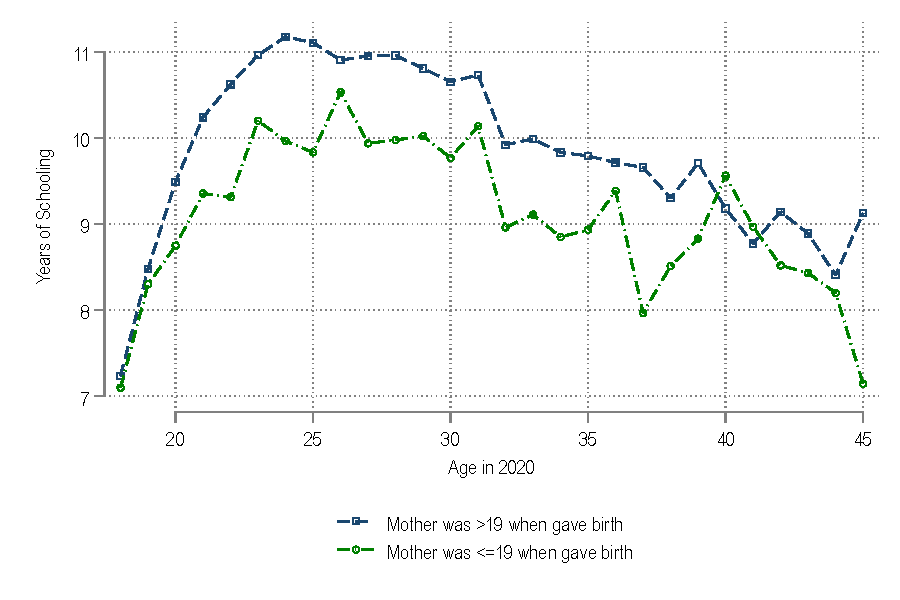
\includegraphics[scale=.8]{output/schooling_dif.pdf}  \\
\end{tabular}\par}
 	 	\vspace{.2cm} %\newline 
\begin{spacing}{0.7}
{\footnotesize{}Notes: This Figure plots the difference is years of schooling between individual whose mother gave birth to them before or after age 20. 
}{\footnotesize\par}
\end{spacing}
\end{centering}
\end{figure}

\begin{table}[H]
\captionsetup{justification=centering}
\begin{centering}
    \caption{Differences in Schooling by Teen Pregnancy Status}
    \label{tab:did}
\par\end{centering}
\begin{centering}
 \scalebox{0.9}{\begin{tabular}{lccc}\hline
& \multicolumn{3}{c}{Years of Schooling} \\ \hline
& (1)  & (2) & (3) \\  \hline
Teen Pregnancy & -0.312 & -0.543 & -0.299  \\
& (0.049) & (0.046) & (0.066)  \\ \hline
Age & No & Yes & Yes  \\
Age Sq & No & Yes & Yes  \\
Female & No & Yes & Yes  \\
Sibiling Group FE & No & No & Yes \\ \hline
\end{tabular}
}
 	\vspace{.2cm} %\newline 
\par\end{centering}
\begin{spacing}{0.7}
{\footnotesize{}Notes:  }
{\footnotesize\par}
\end{spacing}
\end{table}

\begin{figure}[H]
\captionsetup{justification=centering}
\caption{Differences in Probabilities of having a birth disability by Mother Teen Pregnancy Status}
\begin{centering}
{\begin{tabular}{c}
A. Years of Schooling  \\
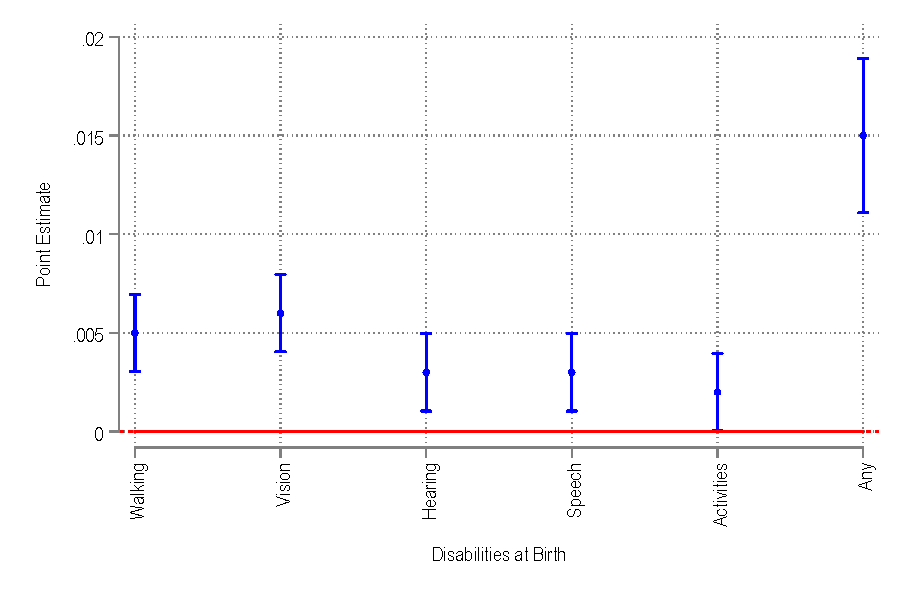
\includegraphics[scale=.8]{output/disabilities_coef.pdf}  \\
\end{tabular}\par}
 	 	\vspace{.2cm} %\newline 
\begin{spacing}{0.7}
{\footnotesize{}Notes: This Figure plots the difference in the probability of being born with a disability between individual whose mother gave birth to them before or after age 20. 
}{\footnotesize\par}
\end{spacing}
\end{centering}
\end{figure}

\end{document}
